\documentclass[UTF8]{article}
\usepackage{ctex}
\usepackage{geometry}
\usepackage{cite}
\usepackage{tikz}
\usepackage{xcolor}
\usepackage{listings}
\usepackage{graphicx}
\usetikzlibrary{graphs, positioning, quotes, shapes.geometric}
\usepackage{url}
\usepackage{threeparttable}
\usepackage{CJK}
\usepackage[colorlinks,
linkcolor=blue,
anchorcolor=blue, 
citecolor=blue,        
]{hyperref}
%\ctexset{bibname=}
\begin{document}
	\title{\vspace{+10pt} \heiti \textbf {基于熵权法的多元线性回归经济增长模型}}
	\author{}
	\date{}
	\maketitle
	\vspace{-70pt}
	\section*{\centering \heiti 摘要}
		\vspace{-20pt}
		~\\\indent 
		\songti
		本文综合考虑影响经济发展的多种因素,建立与劳动人口规模、经济增长起点、资源禀赋、教育、外商投资以及是否有疫情等突发事件有关的经济增长模型。本文模型运用最大归一化处理方法量化各个变量,并利用熵权法计算权重,使得各个因素的评估更加科学。同时通过多元线性回归的方法进行对未来20年经济的预测。本文建模与数据分析所使用的软件为Stata、Excel、Matlab。
		\\\indent 针对建立考虑多因素的经济增长模型的问题,首先从国家统计局官网~\cite{NBS} 根据需要搜集近20年经济数据,对于缺失的数据则使用三次样条插值法和回归方程预测法进行补充,然后利用归一化方法处理这些数据。该模型中自变量与因变量选取的最终目的是使得拟合度高的情况下,自变量与因变量关系的显著性也尽可能科学,符合生活实际。
		\\\indent
		本文模型基于上述考虑最终选取的因变量为年度GDP、年度人均GDP、年度人均GDP增长率。模型参考的各个因素及相关的自变量如下:经济增长起点———前一年GDP;人口规模——15-64岁人口、劳动人口与总人口的比例;资源禀赋——耕地规模、工业企业数量;教育水平——教育经费、九年义务教育普及率、应届普通本科生与专科生毕业或结业人数、应届研究生毕业或结业人数、年度高校入学率、发明专利申请授权数;外商投资——实际利用外商直接投资金额;以新冠和非典为代表的疫情因素——0-1虚拟变量。从上述搜集的数据中进行筛选后,利用熵权法求得权重进而得出各个因素不同年份的标准化评分,最后利用这些数据建立回归模型。
		\\\indent 
		针对预测未来20年教育水平如何影响经济增长和判断经济增长率为 7\% 是否可行的问题,本文使用多元线性回归的方法,在建立模型的基础上分析了教育之于经济增长的重要意义并利用所建立的模型进行预测计算。经过异方差和多重共线性等检验,本模型虽可以忽略异方差影响且回归拟合优度较高,但是自变量间存在着一定的多重共线性与内生性,因此并不能很准确地预估每个自变量的显著性。基于此本文对模型进行了评价。最后根据建立的模型与拟合的结果给出结论并向政府提出实际可行的建议。
		\\
		\\{\heiti 关键词:多重共线性检验\quad 数据拟合\quad 多元回归\quad 多元分析\quad 熵权法\quad 经济增长}
	\newpage
	\section{问题重述}
		\subsection{问题背景}
		\indent 近几十年来,中国经济高速发展的决定性因素经历了显著的改变,历史上中国经济的增长受到两股力量的推动:“人口红利”与劳动力生产效率的提高。
		\\\indent 然而,近年来,中国劳动力的构成发生了变化,中国劳动力的再分配的速率也有所放缓,这无疑威胁到了中国经济的持续高速增长,所以中国若希望其经济保持中高速增长,则需要重视教育因素,从而弥补劳动力规模和劳动生产率的下降。
		\subsection{需要解决的问题}
		\paragraph{问题一}经济的增长与多种因素有关,建立一个模型,该模型可以考虑如下因素:{\heiti 经济增长起点}、{\heiti 劳动人口规模}、{\heiti 资本禀赋}、{\heiti 教育}、{\heiti 其他重要因素}。
		\paragraph{问题二}利用该模型估计未来二十年{\heiti 教育水平}会如何对中国经济发展产生影响,估测未来的{\heiti 增长率}或者{\heiti 收入水平},判断未来人均经济增长人均为 7\% 是否可行,并向政府提出相应的建议。
	\section{问题分析}	
		\subsection{建立多因素影响下的经济增长模型}
		\indent 此问题要求我们建立考虑多种因素的经济增长模型,但经济的增长是一个十分复杂的过程,而且影响经济发展的各种因素都可以用多个变量来衡量,因此本文首先对变量进行多重共线性检验和异方差检验,筛选出可以用于衡量各个因素的变量(图\ref{jjzz})。对于资源禀赋这一相对宽泛的概念,本文选取耕地面积和企业数量两个变量进行评估,此外,由于本模型最终侧重于分析教育影响经济的机理,教育水平的评估涉及更多变量。
		\newpage
		\begin{figure}[htb]
			\centering
			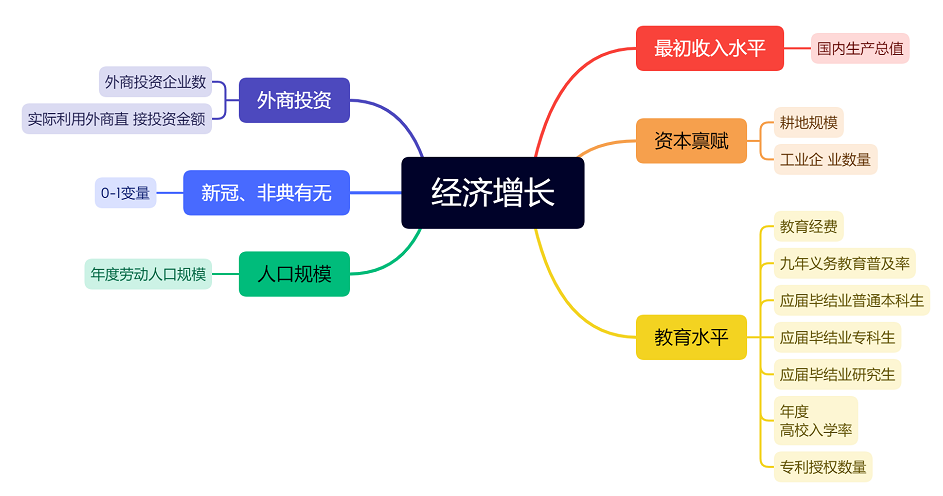
\includegraphics[width=10cm]{pictures/jjzz.png}
			\caption{经济增长分析}
			\label{jjzz}
		\end{figure}
		此后,本文利用在国家统计局官网近20年内的相关数据,首先用三次样条插值法和回归方程预测法补充缺失的数据,然后利用熵权法计算权重,解决各个因素的评估问题。最后运用多元线性回归的方法,建立经济增长的预测模型。在解决本问题过程中所求得的数据和函数为解决第二问奠定了基础。
		\subsection{运用以上模型解决一系列实际问题}
		\subsubsection{预测未来20年教育水平会如何对中国经济增长产生影响}
		本小问需要研究并解释教育水平对经济增长产生影响的机理,这实质上是一个偏相关分析的过程,因为该模型中经济与多种因素相关,并且这一小问中需要特殊地指出教育水平这一因素及其相关变量在模型中是如何影响经济增长的。可以采取控制变量法,说明在其他因素变化趋势保持不变的情况下,教育水平的起伏会怎样影响到经济的发展。
		\subsubsection{未来的经济增长率或收入水平会是多少?}
		本小问需要利用上述模型进行计算,实质上是一个多元回归分析问题,需要利用已知数据选取合适的回归模型进行预测。之后分析预测的结果,定性与定量地指出为什么会有这样的结果,
		\subsubsection{未来20年人均经济增长年均为 7\% 是否可行}
		本小问要考虑一个特定的增长率是否可行,实质上是一个分析预测结果的实际问题,为了解决此问题,只需要利用上一问所得结果进行比较判断,并对误差和置信度与置信区间进行说明即可。
		\subsubsection{向政府建言献策}
		本小问是一个开放性的问题,回答的角度多种多样,但是基于题目背景,应当侧重于从教育角度提相关建议,其他角度为辅,需要通过摆结论-讲依据-说方法的方式提出可靠、可行的建议,建议宜通俗易懂,不宜使用大量公式和数据。对于预测模型可能存在的问题,出错的概率以及一些不可预料的因素也要提及。
	\section{模型假设}
	%\vspace{-20pt}
	\begin{itemize}
		\item 在经济建设中,主要由劳动人口作出贡献,因此用劳动人口数量和劳动人口的占比这两组变量来概括劳动人口规模
		\item 经济发展起点由前一年国内生产总值决定,资源禀赋由耕地面积和工业企业数量决定,教育水平由教育经费、教育的普及率、入学率和毕业生人数等决定
		\item 多重共线性检验后得到的模型,如果其在改进后依然存在严重的多重共线性,则进一步深入分析该模型,判断能不能忽略多重共线性对其的影响
		\item 该经济增长的回归模型是正确设定的
		\item 所有自变量的随机误差项满足正态分布且均值为0,且与相应自变量同方差、不序列相关
	\end{itemize}
	\section{模型主要变量符号及含义}
	\begin{center}
		\begin{threeparttable}
		\setlength{\tabcolsep}{10mm}
		\begin{tabular}{ccc}
		\hline
		序号 & 符号 & 意义\\
		\hline
		1 & Y1 & 国内生产总值\\
		2 & Y2 & 人均国内生产总值\\
		3 & Y3 & 人均国内生产总值增长率\\
		4 & X1 & 实际利用外商直接投资金额\\
		5 & X2 & 年度资源禀赋\\
		6 & X3 & 年度教育水平\\
		7 & X4 & 年度劳动人口规模\\
		8 & X5 & 该年经济发展起点\\
		9 & X6 & 虚拟变量A1\tnote{1}\\
		10 & X7 & 虚拟变量A2\tnote{2}\\
		11 & t & 年份\\
		\hline
		\end{tabular}
	\begin{tablenotes}
		\item [1] 当年无疫情影响经济增长
		\item [2] 当年有疫情影响经济增长
	\end{tablenotes}
\end{threeparttable}
	\end{center}
~\\
	\section{模型建立}
	\vspace{-10pt}
	~\\建模过程可以概括为图\ref{jmgc}
	\begin{figure}[htb]
	\centering
	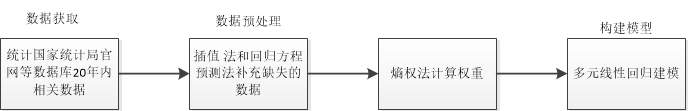
\includegraphics[width=10cm]{pictures/jmgc.png}
	\caption{建模过程}
	\label{jmgc}
	\end{figure}
	\subsection{选取合适的变量}
	\vspace{-10pt}
	~\\本文参考经济学论文~\cite{kaldor1957model}初步选取如下变量并从国家统计局官网\cite{NBS}收集近20年数据
	\subsubsection{经济增长起点}
	国内生产总值是某时期内一个区域的经济生产中产出的全部成果的市场价值,是国民经济核算的核心指标,对于衡量一个国家或者地区的经济状况和发展水平有着重要意义。本文模型拟选取全中国范围为研究对象,并以年为单位,因此选取前一年国内生产总值为衡量最初收入水平的变量。
	\subsubsection{劳动人口规模}
	在衡量人口规模因素对经济发展的影响时,需要考虑劳动的参与率。劳动人口规模是一个国家或地区中具有劳动能力的那部分人口,劳动人口的规模一定程度上反映了一个国家的劳动参与率\cite{ldrk},又因为一般而言劳动能力与人的年龄有着密切的关系,故所有人口中属于劳动适龄范围内的那一部分人口才是劳动人口,男女性劳动适龄范围有所不同,劳动力人口形成了一个国家或地区的劳动力资源。因此劳动人口规模精简地概括了人口规模对经济发展的影响,本文模型选取劳动人口所占比例以及15-64岁人口作为衡量人口规模的变量。
	\subsubsection{资源禀赋}
	资源禀赋可以说是一个很广的概念,但在本题目中不是重点考虑因素,所以本文模型只用少量有代表性的变量衡量。资源禀赋是指一国拥有的各种生产要素,包括劳动力、资本、土地、技术等\cite{caten}。其中劳动力在前一个因素中有涉及,技术的各项衡量指标又与教育水平有很强的线性相关性,与模型假设相悖,因此最终选取全国耕地面积和全国工业企业数量来衡量资源禀赋(图\ref{zybf})。
    	\begin{figure}[htb]
    	\centering
    	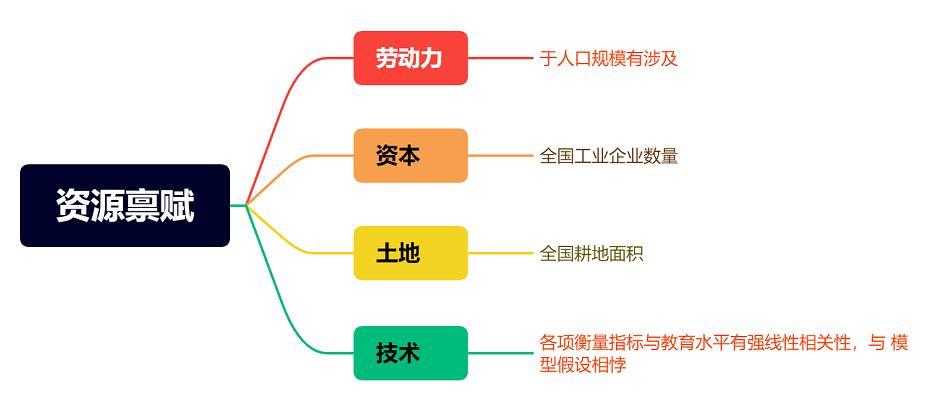
\includegraphics[width=8cm]{pictures/zybf.png}
    	\caption{资源禀赋分析}
    	\label{zybf}
    	\end{figure}
	\subsubsection{教育}
	教育水平是国民接受教育的程度。教育一般分为学前教育、初等教育、中等教育、高等教育四个阶段,其中学前教育与经济发展关系不大,所以主要考虑与另外三个阶段相关的变量。办教育需要人力物力,办多少学校、允许多少人接受教育都取决于一个国家的经济实力与生产力,所以一个国家教育的水平从根本上而言取决有生产力的发展水平与经济水平的高低,生产力水平与经济水平越高,能投入到教育之中的资源就越多,这种资源集中体现为教育经费,所以本模型首先选取教育经费作为变量,经费的投入直接体现了国家对教育的重视程度,并且从根本上决定了一个国家的教育水平。此外,从教育的接受者程度角度,本文模型选取了九年义务教育的普及率作为自变量,从教育机构的角度,本文模型选取了年度高校入学率、专科生/本科生/研究生毕/结业生数量作为自变量,从教育的产出角度,本文模型选取发明专利申请授权数作为自变量。
	\subsubsection{其他因素}
	\paragraph{外商投资}外商的投资对于中国经济的增长也有不小贡献,本文模型选取外商投资企业数来衡量外商投资对于中国经济发展的影响。
	\vspace{-10pt}
	\paragraph{疫情背景}新冠与非典对经济发展的影响之大是全国人民有目共睹的,疫情下有诸多不确定性并且疫情的影响范围波及全球,疫情下经济的发展是另一种状态,因此疫情对经济的影响有这样的特点:改变了经济发展的状态使得经济发展的趋势有了质的不同,因此对于这种性质的因素,我们使用0-1虚拟变量进行衡量、区分。
	\\
	\\\indent
	选取上述变量后作出假设:经济增长和每一个定量变量都应呈正相关,并认为没有疫情的影响的中国经济增长会更快。
	\subsection{利用三次样条插值法补充数据}
	\leftline{首先考虑在STATA上使用三次样条插值法,三次样条插值法公式如下(具体细节不作展开):}
	$$
		S(x)=a_i+b_i(x-x_i)+c_i(x-x_i)^2+d_i(x-x_i)^3
		\label{czgs}
	$$
	\leftline{原始数据中,耕地面积数据缺失(图\ref{ysgdmj})}
	\newpage
	\begin{figure}[htb]
		\centering
		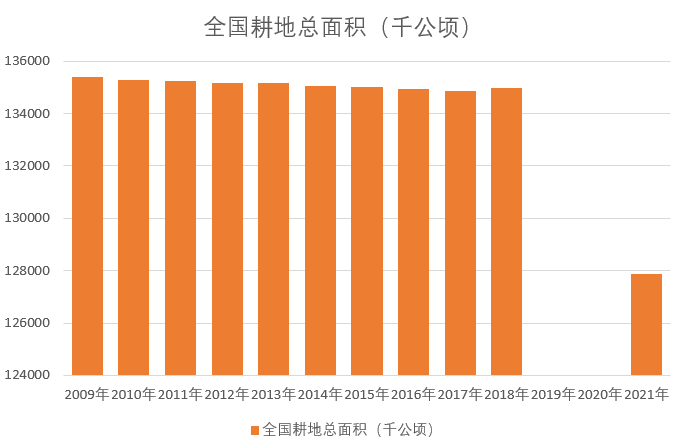
\includegraphics[width=8cm]{pictures/ysgdmj.png}
		\caption{原始耕地面积数据}
		\label{ysgdmj}
	\end{figure}
	\leftline{考虑近20年所有数据利用三次样条插值法补充后,得到的数据统计图如下\ref{bcgdmj}:}
	\begin{figure}[htb]
		\centering
		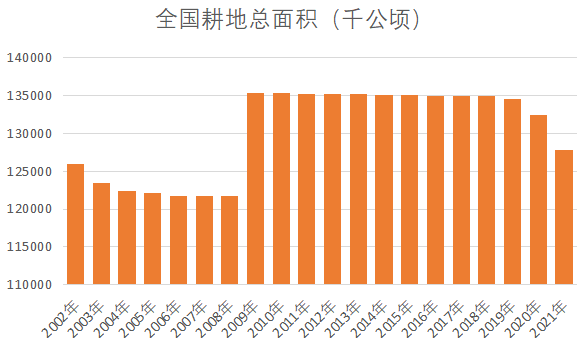
\includegraphics[width=8cm]{pictures/bcgdmj.png}
		\caption{补全后的耕地面积数据}
		\label{bcgdmj}
	\end{figure}
	\leftline{其次考虑回归方程预测法(即普通最小二乘法OLS)补充2021年教育经费数据}
	~\\公式如下:
	$$
	k=\frac{\sum_{i=1}^n x_iy_i-n\bar{x}\bar{y}}{\sum_{i=1}^{n}{x_i}^2-n{\bar{x}}^2}
	$$
	\vspace{+5pt}
	$$
	b=\bar{y}-k\bar{x}
	$$
	\leftline{补充前数据如图\ref{ysjyjf}}
	\newpage
	\begin{figure}[htb]
		\centering
		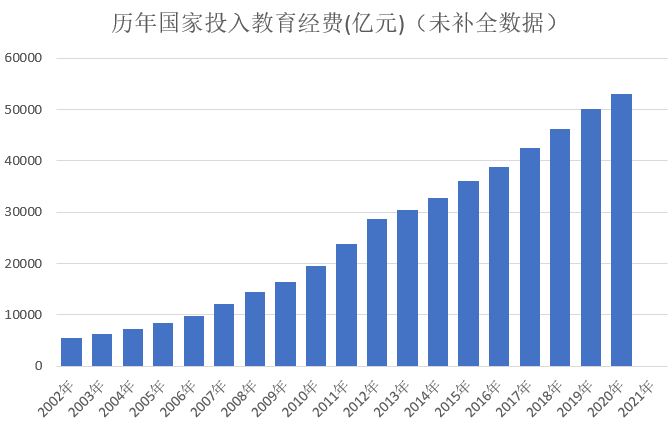
\includegraphics[width=8cm]{pictures/ysjyjf.png}
		\caption{原始教育经费数据}
		\label{ysjyjf}
	\end{figure}
	\leftline{用OLS求得回归方程及其拟合优度为:}
	\vspace{-10pt}
	$$
		y=2789.35x-5583989,R^2=0.98
	$$
	\leftline{代入该公式补充数据后如图\ref{bcjyjf}:}
	\begin{figure}[htb]
	\centering
	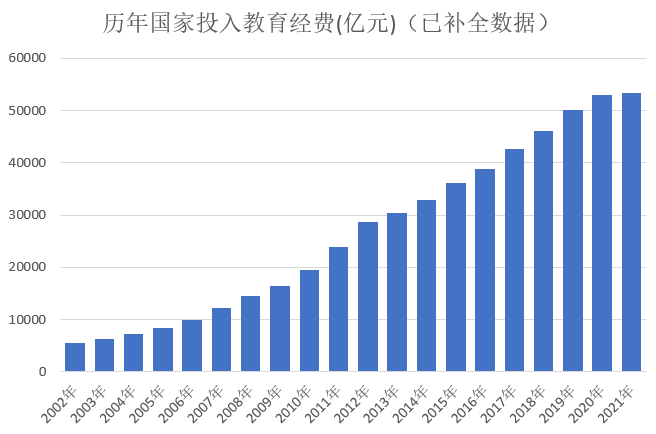
\includegraphics[width=8cm]{pictures/bcjyjf.png}
	\caption{补充后教育经费数据}
	\label{bcjyjf}
	\end{figure}
	\newpage
	\leftline{同理,对于缺失数据的义务教育普及率,补充前如图\ref{ysywjy}:}
	\begin{figure}[htb]
		\centering
		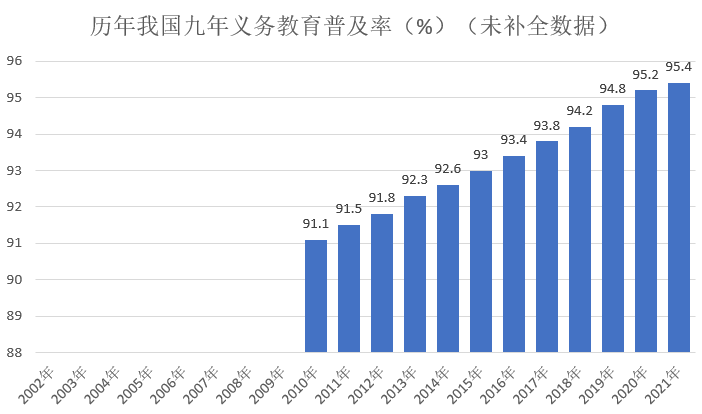
\includegraphics[width=8cm]{pictures/ysywjy.png}
		\caption{原始义务教育普及率数据}
		\label{ysywjy}
	\end{figure}
	\leftline{用OLS求得回归方程及其拟合优度为:}
	$$
		y=0.4024473-717.8747,R^2=0.9971
	$$
	\leftline{代入公式补全后数据后的统计图如下\ref{bcywjy}:}
	\begin{figure}[htb]
	\centering
	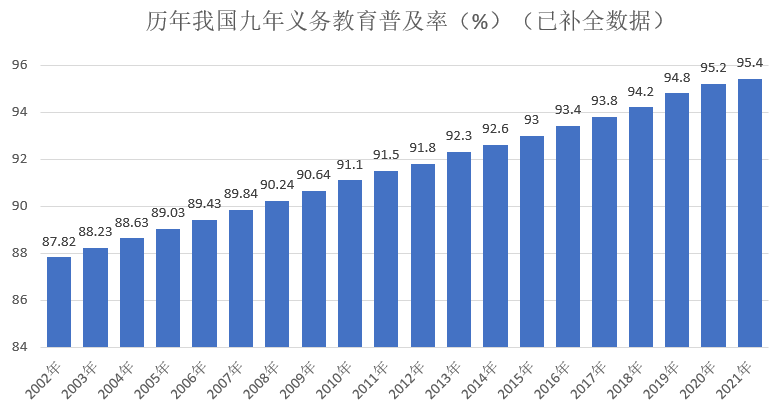
\includegraphics[width=8cm]{pictures/bcywjy.png}
	\caption{补全数据后的义务教育普及率}
	\label{bcywjy}
	\end{figure}
	\subsection{利用熵权法计算权重}
	本文应用熵权法求解的过程参考了论文\cite{sqf}
	\\求解过程如图\ref{sqf}
	\newpage
	\begin{figure}[htb]
	\centering
	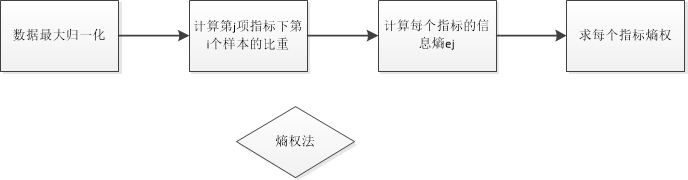
\includegraphics[width=10cm]{pictures/sqf.png}
	\caption{求解过程}
	\label{sqf}
	\end{figure}
	首先利用Matlab对教育的数据进行标准化处理(采取正向指标),理论公式如下:
	$$
	X^{'}_{ij}=\frac{x_{ij}-min(x_j)}{max(x_j)-min(x_j)}
	$$
	以教育为例,标准化矩阵如图\ref{jybzhjz}所示(其余标准化矩阵在支撑材料中),从左到右依次为:国家投入教育经费、九年义务教育普及率、应届普通本科/专科生毕(结)业生数、应届研究生毕(结)业生数、发明专利申请授权数量、该年高校入学率:
	\begin{figure}[htb]
	\centering
	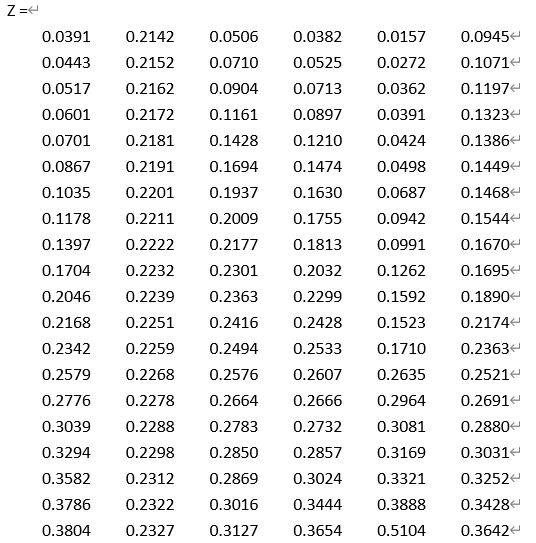
\includegraphics[width=8cm]{pictures/jybzhjz.png}
	\caption{教育水平的标准化矩阵}
	\label{jybzhjz}
	\end{figure}
	\\然后求得各项指标的信息熵,定义:
	$$
	p_{ij}=\frac{X^{'}_{ij}}{\sum_{i=1}^{n}X^{'}_{ij}}
	$$
	特殊地,若$p_{ij}=0$,则添加定义如下
	$$
	\lim_{x\to 0}p_{ij}\ln p_{ij}=0
	$$
	于是可以计算各项指标的信息熵:
	$$
	E_j=-\frac{1}{\ln n}\sum_{i=1}^{n}p_{ij}\ln p_{ij}
	$$
	通过信息熵可以利用如下公式计算n个指标的权重:
	$$
	W_{j}=\frac{1-E_{j}}{n-\sum_{i=1}^{n}E_{i}}	
	$$
	在Excel中计算得各项权重如图\ref{jyqz}:
	\begin{figure}[htb]
	\centering
	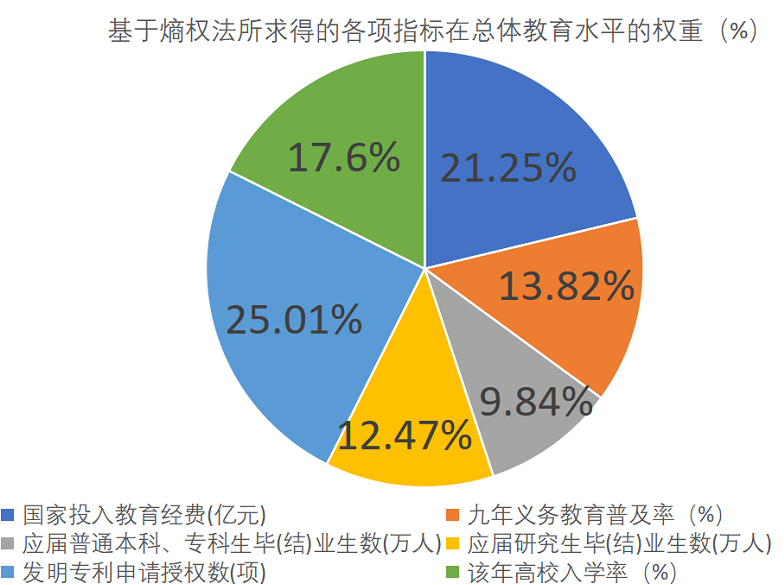
\includegraphics[width=8cm]{pictures/jyqz.png}
	\caption{教育水平的各项权重}
	\label{jyqz}
	\end{figure}
	\\同理可以求得劳动力规模的权重如图\ref{ldlqz}:
	\newpage
	\begin{figure}[htb]
	\centering
	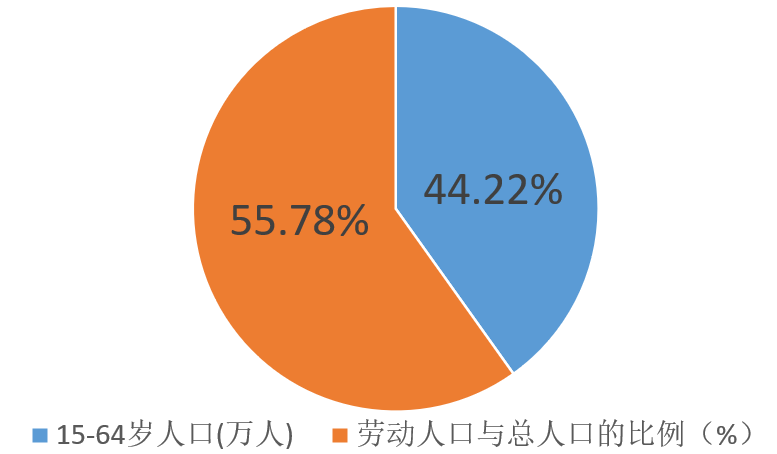
\includegraphics[width=8cm]{pictures/ldlqz.png}
	\caption{人口规模的各项权重}
	\label{ldlqz}
	\end{figure}
	资源禀赋的各项权重如图\ref{zybfqz}:
	\begin{figure}[htb]
	\centering
	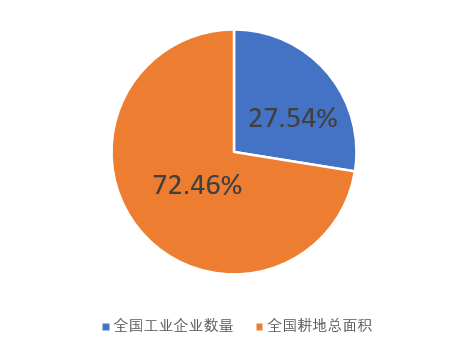
\includegraphics[width=8cm]{pictures/zybfqz.png}
	\caption{资源禀赋各项权重}
	\label{zybfqz}
	\end{figure}
	\\利用上述权重数据及标准化后的数据可以得到各项的标准化评分,以资源禀赋与人劳动口规模得分为例,各年的得分情况如图\ref{zybfdf}、\ref{rkgmdf},详细得分数据在附录第I部分。
	\newpage
	\begin{figure}[htb]
		\centering
		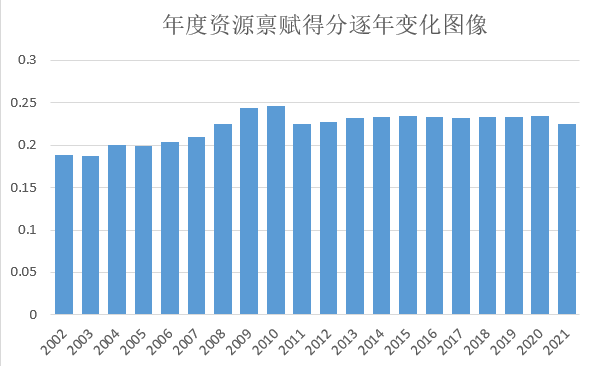
\includegraphics[width=8cm]{pictures/zybfdf.png}
		\caption{资源禀赋各年得分}
		\label{zybfdf}
	\end{figure}
	\begin{figure}[htb]
		\centering
		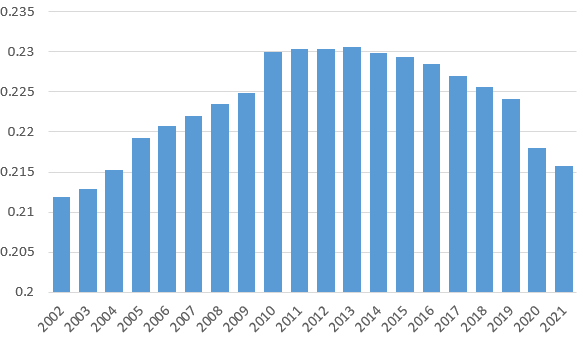
\includegraphics[width=8cm]{pictures/rkgmdf.png}
		\caption{人口规模各年得分}
		\label{rkgmdf}
	\end{figure}
	\subsection{建立多元线性回归模型}
	接下来,我们以X1-X7为自变量,Y1-Y3为因变量,建立经济增长的模型,先以Y1为因变量为例,代入2002年至2021年20年的数据,使用STATA软件进行计算得到如图\ref{y1}结果
	\newpage
	\begin{figure}[htb]
	\centering
	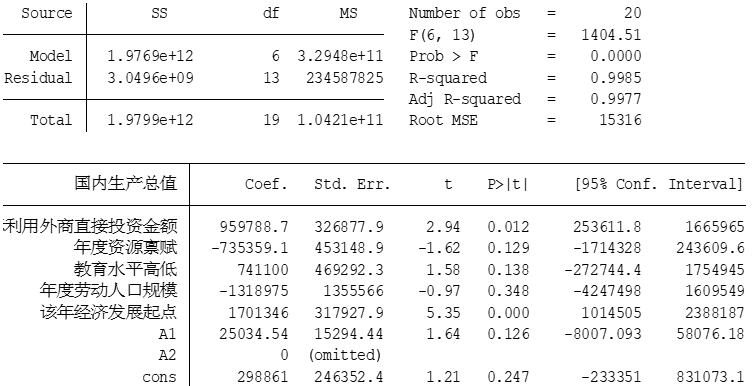
\includegraphics[width=12cm]{pictures/y1.png}
	\caption{STATA回归分析结果}
	\label{y1}
	\end{figure}
	\vspace{-10pt}
	\paragraph{总体拟合效果}由上图的计算结果可知,在检验该回归是否有意义时,构建了一个F统计量F(6,13),该F统计量的原假设$H_0$为“$X_1$到$X_7$ 前的系数均为0”该统计量的检验值为1404.51,它所对应的P值为小于0.01,这说明在99\%的置信水平下,应当拒绝原假设并认为“ 前的系数显著异于0”这表明我们所构建的多元线性回归是有意义的。
	由上图的计算结果可知,回归方程拟合优度$R^2=0.9985$ ,调整后的拟合优度$R^2=0.9977$,两者都与1非常接近,因此可以认为该回归的整体拟合效果非常好。
	\\
	\\补充说明:关于拟合优度和谓整后的拟合优度:一般情况下我们引入的自变量越多,回归方程的拟合优度会变大。但我们倾向于使用调整后的拟合优度,如果新引入的自变量对SSE(残差平方和)的减少程度特别少,那么调整后的拟合优度反而会减小。
	$$
	R^2=1-\frac{SSE}{SST} \indent R^2_{adjusted}=1-\frac{SSE\times(n-1)}{SST\times(n-k-1)}
	$$
	\paragraph{对于自变量前正负号的初步分析}
	注意观察到自变量$X_1$、$X_3$、$X_5$、$X_6$前的系数为正,这表明外商投资金额越大、国家教育水平越高、国家经济发展的起点越高,中国年度国内生产总值就越大。也可以说明在其他条件不变的情况下,无疫情影响下的中国一年的国内生产总值,大于有疫情影响下的中国一年的国内生产总值。这一结论是符合我们预测的,也是符合经济学原理的。而根据计算结果,我们可以注意到$X_2$和$X_4$前的系数为负数,但是这可以说明一国的资源禀赋和该国的劳动人口规模大小,与该国年度国内生产总值大小呈负相关吗?凭回归结果可以得出“为了实现经济的更快增长,应该让这两个指标越低越好”这样的反常结论吗?
	\paragraph{对于$X_2$、$X_4$随年份变化的图像的分析}
	根据图\ref{zybfdf}以及使用Stata算得的年度资源禀赋与人口规模的线性拟合优度(如图\ref{zybfnhyd}、\ref{rkgmnhyd})。
	\begin{figure}[htb]
	\centering
	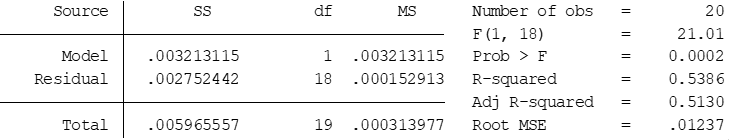
\includegraphics[width=12cm]{pictures/zybfnhyd.png}
	\caption{资源禀赋线性拟合优度}
	\label{zybfnhyd}
	\end{figure}
	\begin{figure}[htb]
	\centering
	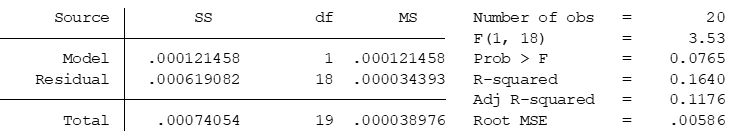
\includegraphics[width=12cm]{pictures/rkgmnhyd.png}
	\caption{人口规模线性拟合优度}
	\label{rkgmnhyd}
	\end{figure}
	\\年度资源禀赋得分和年度劳动人口规模的得分并不是逐年单向变化的,资源禀赋和劳动力规模得分与时间的线性关系不明显,而中国的年度国内生产总值是随着时间的推移逐步递增的。由Stata计算可得,年度资源禀赋与年份的回归拟合优度为$R^2_{1}=0.5386$、年度劳动人口规模与年份的回归拟合优度$R^2_{2}=0.1670$。上述两个变量的拟合优度都不够接近1,表明其线性拟合效果不佳。进一步佐证了上述两变量与时间非线性相关。
	\paragraph{对于这种现象的解释}首先我们要再一次强调我们是如何得到“年度资源禀赋得分”“和年度人口规模得分”这两个自变量的。年度资源禀赋的总分由两部分组成:分别是占比27.54\%的“工业企业单位数(个)”和占比72.46\%的“全国耕地总面积(千公顷)”这两组数据是宏观数据,能反映中国参与经济建设的土地面积和工厂数目,但是它们并不能反映出每一块土地的利用效率和每一家工业企业的生产效率,也就是说自变量$X_2$的变化不能反映出近20年中国工农业生产效率的变化。年度劳动人口规模的得分亦由两部分组成:分别是占比55.78\%的“15-64岁数量(万人)”和占比44.22\%的“劳动人口与总人口的比例(\%)”这两组数据同上述的两组数据一样,都是宏观数据,它们加权和得到的自变量$X_4$可以反映出近20年来中国劳动人口数量和中国总体人口结构的变化,但是并不能反映出每一个劳动者个体的生产效率及其经济建设能力。
	\\\indent 
	放眼世界许多发达国家的经济增长史,国家的工农业生产效率和劳动者素质,无不是随着发展水平的提高而逐步提高的。在经济发展的进程中,国家会逐步淘汰落后产能、倒闭生产效率低下的企业以促进社会资源的合理分配;当经济发展达到了一定水平以后,政府会提倡绿色健康可持续发展,会颁布法律法规进行生态修复、污染治理,而此类政策会在一定程度上减少该国企业、耕地、牧场的数量;经济增长带来人们的生活水平的提高后,人们的思想观念也会在一定程度上发生改变,“少生晚生甚至不生”的观念也被更多的年轻人所接受,这在一定度上直接加剧了人口老龄化社会的形成,也在一定程度上减少了一国的劳动人口数量。对这些现象的解释是:劳动人口、工业企业、农业用地的数量的减少,是经济发展到特定阶段的产物。因为随着劳动者素质和工农业生产效率的提高,经济也随之加速增长,而经济的增长会反过来刺激对落后产能的淘汰和对资源的保护,会反过来影响劳动者的思想观念。这也会最终导致劳动人口、工业企业、农业用地的数量的减少。
	对于中国,上述结论一样是适用的。早在在2002年一月,国务院西部开发办公室就召开工作电视电话会议,确定全面启动退耕还林工程;2003年我国更是把科学发展观上升为党的重大战略思想,树立全面、协调、可持续的发展观。国家统计局数据表明,近20年我国全国常住人口出生率呈下降趋势,人口老龄化的社会问题日益严俊。我国劳动人口、工业企业、农业用地数量的减少,正是我国经济发展到一定阶段的产物。
	\\\indent 
	综上所述,从生活实际出发,$X_2$和$X_4$前的系数为负也是可以经济学原理解释的。
	\subsection{以$Y_2$为因变量}
	模型以$Y_2$为因变量时,分析过程和以$Y_1$为因变量时类似。
	\newpage
	\leftline{$Y_2$为因变量的回归分析结果如图\ref{nhjg3}:}
	\begin{figure}[htb]
	\centering
	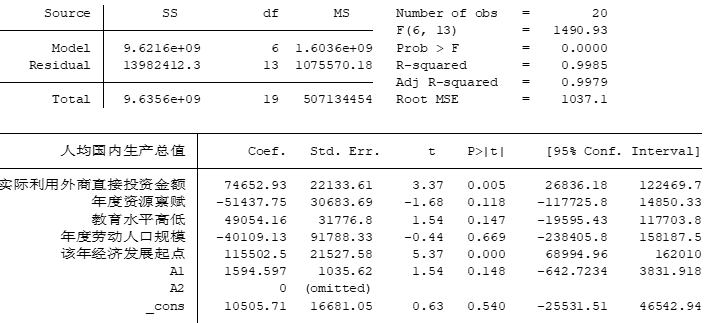
\includegraphics[width=8cm]{pictures/nhjg3.png}
	\caption{STATA回归分析结果}
	\label{nhjg3}
	\end{figure}

	\leftline{$Y_3$近20年变化曲线如图\ref{rjgdp1}:}
	\begin{figure}[htb]
	\centering
	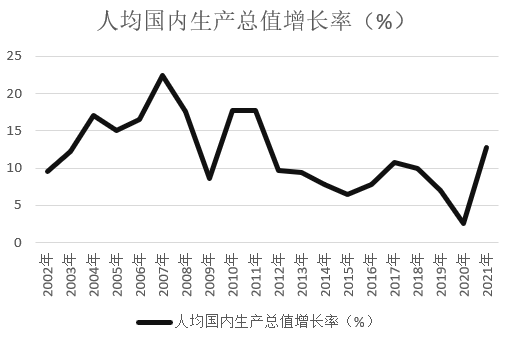
\includegraphics[width=5cm]{pictures/rjgdp1.png}
	\caption{人均GDP增长率曲线}
	\label{rjgdp1}
	\end{figure}
	\leftline{$Y_3$为因变量回归分析结果如图\ref{nhjg5}:}
	\begin{figure}[htb]
	\centering
	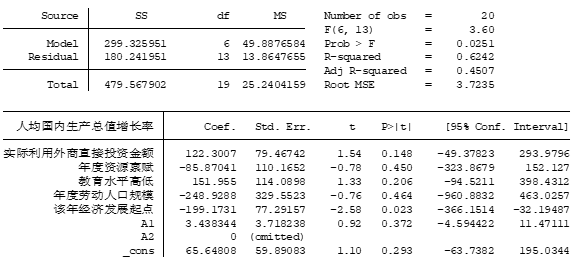
\includegraphics[width=7cm]{pictures/nhjg5.png}
	\caption{STATA回归分析结果}
	\label{nhjg5}
	\end{figure}
	\section{模型的检验与修正}
	对模型的检验过程如下,先以Y1为因变量进行检验。
	\subsection{异方差检验}
	参考研究论文\cite{white},本文模型中异方差检验方法采用White检验,White检验是一种异方差检验方法。一般先将最小二乘估计残差的平方对模型的解释变量、解释变量平方以及解释变量交叉乘积进行回归,然后根据回归方程显著性判断是否存在异方差性。怀特检验的优点是不需要排序,且适合任何形式的异方差。
	
	选择数据使用普通最小二乘法进行多元线性回归后,使用White检验法检验数据的扰动项是否异方差,使用Stata计算检验得到的数据表格如图\ref{yfcjy1}
	\begin{figure}[htb]
	\centering
	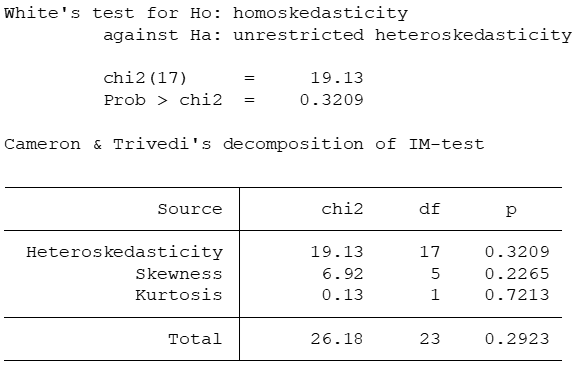
\includegraphics[width=8cm]{pictures/yfcjy1.png}
	\caption{White检验结果}
	\label{yfcjy1}
	\end{figure}
	\\由上图\ref{yfcjy1}计算数据可知,在检验数据的扰动项是否存在异方差时,构建了一原假设为“扰动项存在异方差”的卡方分布chi2(17),该统计量的检验值为19.13,其对应的P值为0.3209。这表明在95\%的置信水平下应当拒绝原假设,认为扰动项不存在异方差。因此使用普通最小二乘法的进行回归预测是合适的。
	\subsection{显著性检验}
	在检验每一个自变量与因变量的关系是否显著时,构造了6个t分布检验。由Stata计算结果可知, 的检验结果所对应的P值分别小于0.05和0.01,这表明在95\%的置信程度上这两个自变量与 显著相关,其中 与与 显著相关的置信水平甚至达到了99\%。这表明外商投资和经济增长起点对某年中国年度GDP影响最为显著,而剩余的自变量对中国年度GDP影响不显著。以有无疫情影响为例,诚然近三年疫情对于全世界经济的冲击十分巨大的,造成了许多企业倒闭、许多劳动者失业,同时旅游业餐饮服务业等多个行业也受创。但是从整个中国的角度来考虑,疫情的出现并没有很大程度上阻碍中国年度国内生产总值的增长,疫情时代我们的经济增长势头还是较为良好的。
	\subsection{对于上述变量显著性检验结果的分析}
	在第一次选择自变量进行回归拟合后,我们可以得出以下结论:
	\\\indent
	(1)中国年度国内生产总值的增长与外商投资和发展起点的相关性显著,这启示我们经济建设应当把引入外商投资作为重中之重。但是这一结论在中国现国情下是不适用的。
	\\\indent
	(2)中国年度国内生产总值的大小与教育发展水平程正相关,但是教育水平高低与中国年度国内生产总值大小并不显著相关,表明教育的发展不会显著提高中国的年度国内生产总值。这一结论与我国的“科教兴国”的国家发展战略思想相悖,与党中央提出的“教育在经济社会发展和民族振兴中具有先导性、基础性、全局性地位”理念相悖。
	\\\indent
	究其原因,是因为各个自变量之间存在严重的多重共线性。
	\\\indent
	虽然变量之间存在的多重共线性不会很大上程度影响多元回归的整体拟合优度,但会导致各个自变量前的系数预测不准确,得出“某一自变量与因变量不显著相关”的结论,而这样得出的结论可能是不符合预期或是不符合现实的。
	\subsection{多重共线性检验}
	~\\下图\ref{vif}是利用Stata计算得到的各个自变量的方差膨胀系数:$VIF=\frac{1}{1-R^2_{i}}$
	\begin{figure}[htb]
	\centering
	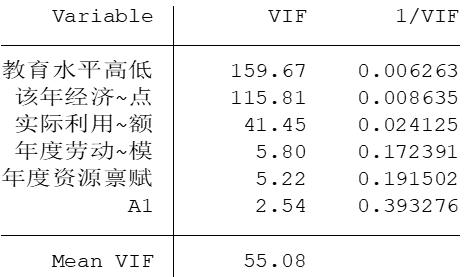
\includegraphics[width=8cm]{pictures/VIF.png}
	\caption{各个自变量的VIF}
	\label{vif}
	\end{figure}
	\\大量数学研究经验表明,当样本中最大的自变量系数的方差膨胀系数大于10时,则认为该回归方程存在严重的多重共线性。由数据可知拟合该经济增长的回归方程存在严重的多重共线性
	一般情况下对于多重共线性的处理有如下方法:
	\\(1)如果不关心具体变量的回归系数,而只关心整个方程预测被解释变量的能力,则通常可以 不必理会多重共线性(假设整个方程是显著的)。这是因为,多重共线性的主要后果是使得对单个变量的贡献估计不准,但所有变量的整体效应仍可以较准确地估计。
	\\(2)如果关心具体的回归系数,但多重共线性并不影响所关心变量的量著性,那么也可以不必理会。即使在有方差膨张的情况下,这些系数依然显著;如果没有多重共线性,则它们只会更加显著。
	\\(3)如果多重共线性影响到所关心变量的显著性,则需要增大样本容量,或剔除导致严重共线性的变量。但是轻易删除变量,可能会有进一步带来内生性的影响。这时候也可以考虑对模型设定进行修改。
	\subsection{自变量的重新考虑与筛选}
	在一开始进行自变量的选择和数据收集时,考虑到穷国和富国的经济可能以不同的方式和速度增长,因此把“该年经济增长起点”作为一个单独的自变量,认为其是影响经济增长的重要因素之一。我们在选择数据衡量“经济增长起点高低”时选择的是去年的国内生产总值,这确实可以衡量经济增长起点的高低,但这在很大程度上也会反映出该国的劳动者素质、科技水平的高低等等元素,因此我们剔除了该自变量再一次使用普通最小二乘法进行了回归,结果如图\ref{nhjg2}:
	\newpage
	\begin{figure}[htb]
		\centering
		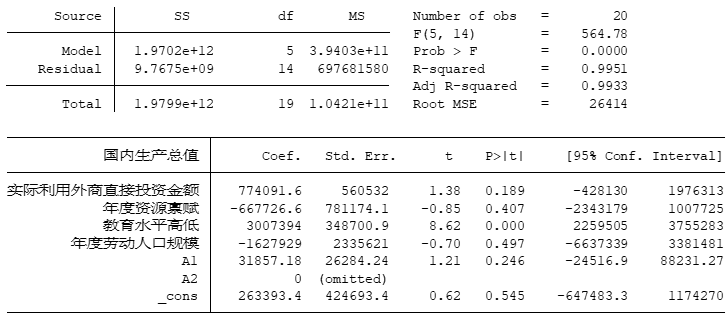
\includegraphics[width=12cm]{pictures/nhjg2.png}
		\caption{新的拟合结果}
		\label{nhjg2}
	\end{figure}
	\leftline{再次检验多重共线性得到VIF如图\ref{vif2}:}
	\begin{figure}[htb]
		\centering
		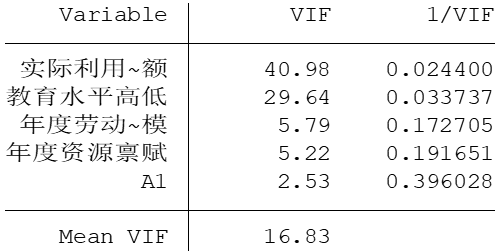
\includegraphics[width=8cm]{pictures/VIF2.png}
		\caption{新的各个自变量的VIF}
		\label{vif2}
	\end{figure}
	\leftline{得到异方差数据如图\ref{yfcjy2}:}
	\begin{figure}[htb]
		\centering
		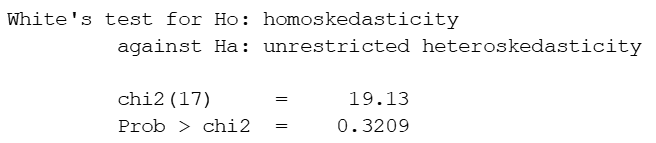
\includegraphics[width=10cm]{pictures/yfcjy2.png}
		\caption{新的异方差检验结果}
		\label{yfcjy2}
	\end{figure}
\newpage
	由数据可得,可以认为调整后的回归方程的扰动项不存在异方差,但是其依然存在多重共线性,对此做出如下考虑:
	\\(1)考虑到该回归的整体拟合优度极佳,运用此模型可以很好地预测未来一段时间中国的年度国内生产总值。
	\\(2)考虑到本题要求我们特别分析“教育水平高低”对经济增长快慢的影响,而这种建模方式可以保证该自变量与因变量的相关性显著。
	\\(3)考虑到增加自变量数据样本的难度较高,且盲目增加自变量可能会影响到重要变量“教育水平高低”的显著性,从而导致偏离题意。
	\\(4)考虑到此时若使用向后逐步回归法,确实可以消除回归方程的多重共线性,但是这样做被剔除的自变量数目过多,只会剩下一到两个自变量。这样的模型必然存在严重的内生性,认为其不具有研究价值。
	综上所述,选择不理会该回归存在多重共线性。
	\subsection{小结}
	在建立年度国内生产总值增长的数学模型时,我们首先对可能影响GDP的变量进行了统计和筛选,最终选择了$X_1$到$X_7$七个自变量。第一次回归加入了所有预想的自变量,最终得到了一个通过了异方差检验的、整体拟合度很高的回归方程。但是后续分析中我们发现该回归依然存在严重的多重共线性,使得我们关心的自变量 与 的相关性不显著。因此我们剔除了一个自变量 再重新拟合回归,最终也得到了一个整体拟合度很高的回归方程,且 与 是显著相关的。对其进行异方差和多重共线性的检验后,我们认为剔除了自变量 再拟合回归的模型更加科学合理。虽然相比之前,整体拟合优度有所下降,但是在分析数据时可以忽略该回归存在的多重共线性,而最初建立的模型因为多重共线性导致各个自变量前的系数预测偏差很大。
	\\\indent
	二者中更科学合理的回归模型表明,无论是最近20年还是未来20年,教育对于经济发展有着至关重要的作用,这一结论是符合假设预期的;对于最初建立的回归模型,认为其不能准确反映出各个自变量与因变量的相关性是否显著。但是在对未来数据的预测和估计上,由于最初建立的模型的整体拟合优度更高,且多重共线性不影响所有变量的整体效应,所以用该回归模型预测数据更加准确。
	\subsection{$Y_2$与$Y_3$为因变量的模型检验与修正}
	\leftline{首先在剔除自变量$X_5$前进行多重共线性检验,结果如图\ref{vif3}:}
	\begin{figure}[htb]
	\centering
	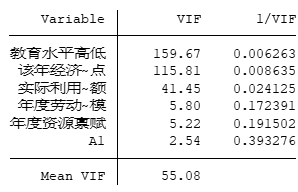
\includegraphics[width=7cm]{pictures/VIF3.png}
	\caption{多重共线性检验结果}
	\label{vif3}
	\end{figure}
	\leftline{剔除自变量$X_5$前进行异方差检验,结果如图\ref{yfcjy3}}
	\begin{figure}[htb]
		\centering
		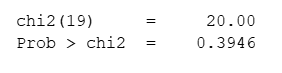
\includegraphics[width=7cm]{pictures/yfcjy3.png}
		\caption{异方差检验结果}
		\label{yfcjy3}
	\end{figure}
	\newpage
	\leftline{在剔除自变量$X_5$后多重共线性检验结果如图\ref{vif4}:}
	\begin{figure}[htb]
		\centering
		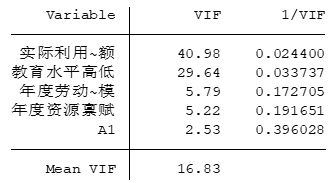
\includegraphics[width=7cm]{pictures/VIF4.png}
		\caption{多重共线性检验结果}
		\label{vif4}
	\end{figure}
	\leftline{在剔除自变量$X_5$后异方差检验结果如图\ref{yfcjy4}:}
	\begin{figure}[htb]
		\centering
		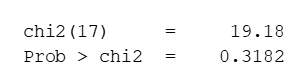
\includegraphics[width=7cm]{pictures/yfcjy4.png}
		\caption{异方差检验结果}
		\label{yfcjy4}
	\end{figure}
	\paragraph{对数据的分析}
	~\\\indent(1)在检验两种回归是否都有意义(即验证自变量前面的系数是否都为0)时,所构建的两种F分布对应的P值均小于0.01,这表明在99\%的置信水平下。两种回归都是有意义的。
	\\\indent(2)当把 全部作为自变量时,所得回归整体的拟合优度 ,调整后的拟合优度 ;当把自变量 剔除后再进行回归,得到的回归整体的拟合优度 ,其调整后的拟合优度 。这表明两种回归的整体拟合效果都非常好。
	\\\indent(3)在进行异方差和多重共线性的检验后,计算结果表明两种回归都可以认为扰动项不存在异方差。但两种回归都依然存在严重的多重共线性,其中剔除自变量 后的回归的多重共线性明显减弱,在分析各个自变量与 的相关性是否显著上,使用后者更为准确。
	\\\leftline{$Y_2$为因变量时剔除自变量$X_5$的回归分析结果如图\ref{nhjg4}:}
	\begin{figure}[htb]
	\centering
	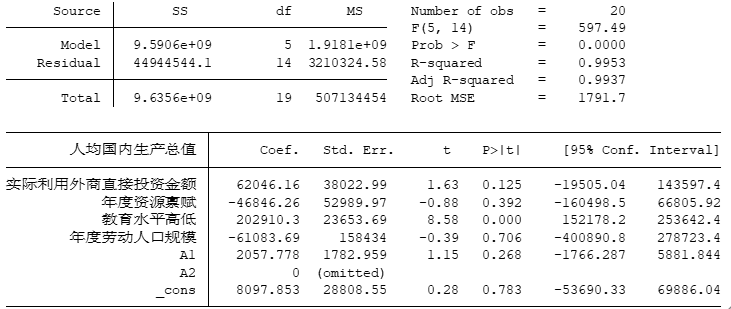
\includegraphics[width=12cm]{pictures/nhjg4.png}
	\caption{STATA回归分析结果}
	\label{nhjg4}
	\end{figure}
	\newpage
	\leftline{$Y_3$为因变量时剔除自变量$X_5$回归分析结果如图\ref{nhjg6}:}
	\begin{figure}[htb]
		\centering
		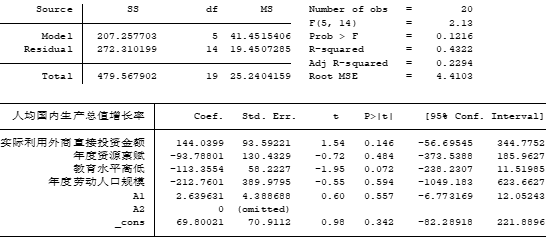
\includegraphics[width=12cm]{pictures/nhjg6.png}
		\caption{STATA回归分析结果}
		\label{nhjg6}
	\end{figure}
	由以上结果可知,$Y_3$与时间不呈明显线性关系,剔除自变量 前后的回归整体拟合优度均小于0.7。认为 与各个自变量之间不是简单的线性关系,用该方程去预测未来数据是非常不准确的,因此认为该模型不具有研究价值。
	\paragraph{小结}
	~\\\indent
	由上文分析可知,在预测未来几年中国的年度人均国内生产总值时,由于两种回归的拟合优度都很接近1,因此可以使用它们中的任意一种进行数据的预估,注意到第一种回归的拟合优度更大一点,因此选择第一种回归进行数据的预测更为准确可靠。
	\\\indent 但是在分析各个自变量与因变量的相关性是否显著时,应当选用剔除了自变量 的回归分析更加科学合理:这是因为剔除了变量 后,回归的多重共线性明显减弱,但依然保证了非常好的整体拟合效果。分析回归结果后可以得出与前者相似的结论:无论是最近20年还是未来20年,教育对年度人均国内生产总值的增长起到了至关重要的作用,应当大力发展教育以推动经济高质量发展。
	\newpage
	\section{模型求解}
	\subsection{建立$Y1$、$Y_2$随时间变化的线性回归方程}
	\leftline{GDP总值如图\ref{nhgdp}:}
	\begin{figure}[htb]
		\centering
		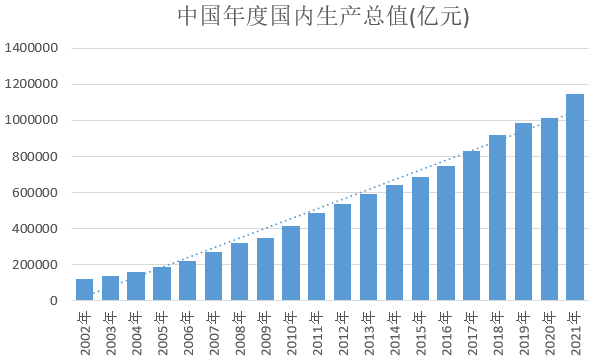
\includegraphics[width=8cm]{pictures/nhgdp.png}
		\caption{$Y_1$回归方程}
		\label{nhgdp}
	\end{figure}
	\leftline{人均GDP如图\ref{nhrjgdp}:}
	\begin{figure}[htb]
		\centering
		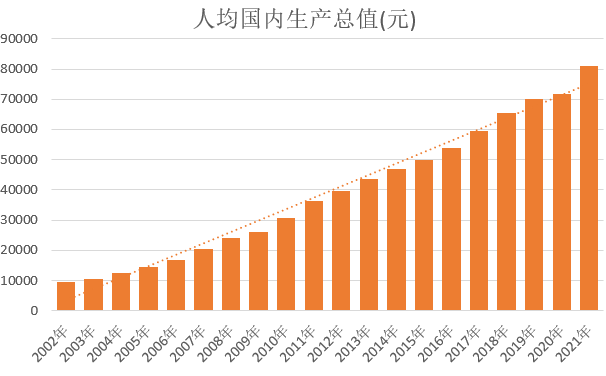
\includegraphics[width=8cm]{pictures/nhrjgdp.png}
		\caption{$Y_2$回归方程}
		\label{nhrjgdp}
	\end{figure}
	对以上两个因变量分别进行回归分析得如图\ref{nhjg7}结果:
	\newpage
	\begin{figure}[htb]
	\centering
	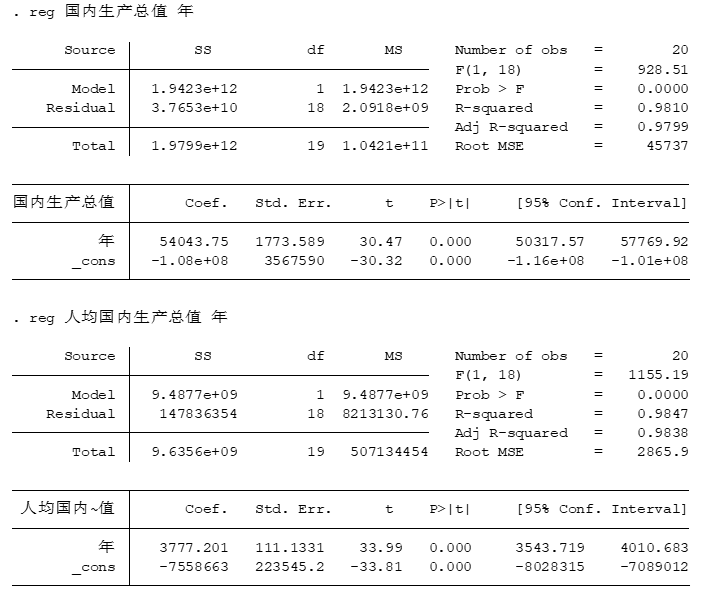
\includegraphics[width=12cm]{pictures/nhjg7.png}
	\caption{回归分析结果}
	\label{nhjg7}
	\end{figure}
	由图像和Stata的计算结果可知,$Y_1$和$Y_2$与时间的线性相关性较强,两回归模型的拟合优度均超过了0.98,可以认为拟合效果很好,可以使用该回归方程预测未来20年的经济增长趋势。 $Y_1$和$Y_2$随时间变化的方程分别如下:
	$$
		Y_1=54043.75t-1.08\times10^8
	$$
	$$
		Y_2=3777.201t-7558663
	$$
	利用回归方程可以预测未来20年后经济增长情况如图\ref{ycjj1},\ref{ycjj2},\ref{ycjj3}:
	\vspace{-2cm}
	\begin{figure}[htb]
	\centering
	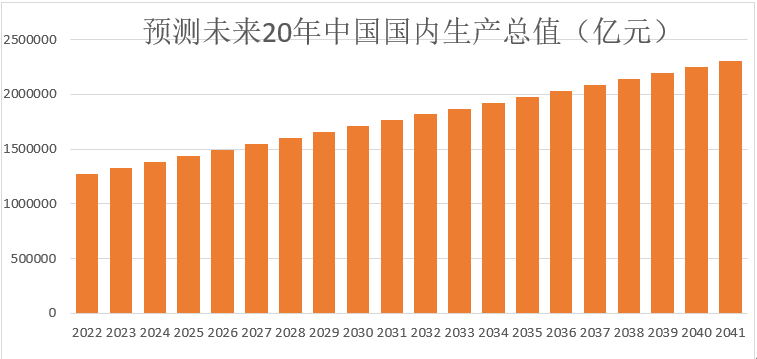
\includegraphics[width=10cm]{pictures/ycjj1.png}
	\caption{预测GDP}
	\label{ycjj1}
	\end{figure}
	\begin{figure}[htb]
	\centering
	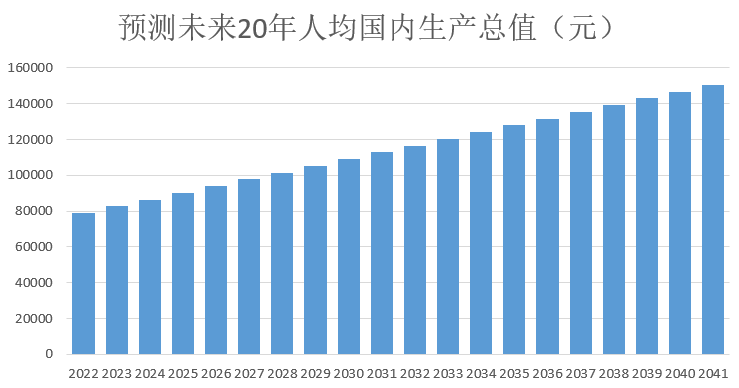
\includegraphics[width=10cm]{pictures/ycjj2.png}
	\caption{预测人均GDP}
	\label{ycjj2}
	\end{figure}
	\begin{figure}[htb]
	\centering
	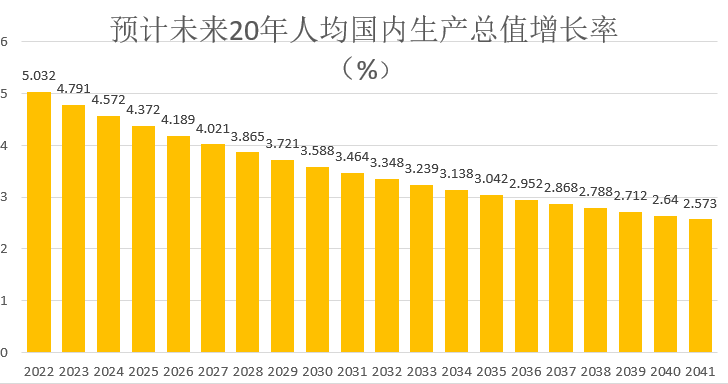
\includegraphics[width=10cm]{pictures/ycjj3.png}
	\caption{预测人均GDP增长率}
	\label{ycjj3}
	\end{figure}
\newpage
~\\由图\ref{ycjj1}、\ref{ycjj2}可知,预计未来20年,我国的经济会稳步增长,经济增长将会保持一个较好的势头。
\\\indent \newpage 但从图\ref{ycjj3}的预测的数据来看,未来20年国内人均GDP的增长速度将会减慢,人均GDP的达不到7\%的年增长速度。然而这并不代表未来中国的经济发展将会滞缓,因为在经济发展的同时,全国的人口数目也会逐步上升;且当发展基数足够大的时候,不高的增长率也可以说明其增长量很大。
\\\indent
综上所述,预测未来20年我们中国的经济将会保持健康平稳地发展,这种健康平稳体现在总体保持增长趋势,增长速度在一定范围内,人民也可以共享发展成果,生活更加富裕。立足当下,虽然疫情不知道什么时候才能结束,但是疫情不会阻挡中国发展的脚步,中国人民众志成城,定会克服困难战胜疫情。

	\newpage
	\section{模型评价}
	\subsection{优点}
	\begin{itemize}
		\item 自变量的选择比较科学,每一个自变量的选取或者剔除都有理可循且基本不会相互覆盖。
		\item 自变量的选取比较全面,基本上能涵盖对经济发展最为重要的几个因素。
		\item 模型进行了严格的检验,如异方差检验中的White检验、多重共线性检验与显著性检验。虽然最后的确定的回归模型依然存在多重共线性,但是分析后认为可忽略其对整体的影响。
		\item 尊重客观事实,模型的建立全过程都是以客观数据为基础。
		\item 可以忽略异方差的影响,异方差是相对于同方差而言的,它意味着误差项的方差不为常数,而同方差是本模型的一个重要假设。
	\end{itemize}
	\subsection{缺点}
	\begin{itemize}
	\item 在多重共线性检验后仍有存在一定相似关系,不能完全独立,即自变量仍然存在着一定的多重共线性
	\item 由于经济增长的模型较为复杂,影响经济增长的因素非常多,所以该模型仍然存在着一定的内生性
	\item 大多数自变量的选取仅是选取代表性强的几个,选取的变量不能完整地概括某个因素的整体水平
	\item 一些自变量的变化情况与预期不符,如资源禀赋与时间非线性相关,因此建立的模型不能很好地衡量每一个自变量的显著性
	\end{itemize}
	\subsection{改进方法}
	一方面,可以选取更加合适的变量来进行建模,无论是哪一个方面的因素,都有大量的数据可供选择,因此,总会有更合适的变量能恰到好处地平衡各个方面且足够全面,降低内生性与多重共线性并提高模型的灵敏性与鲁棒性。另一方面,从根本上说,本模型所具有的局限性是线性模型所共有的,因此,若想从根本上改进,则不能采用原有的线性模型,应当另选其他合适的模型。
	\section{给政府的建议}
	如今我国若希望保持经济高速增长、经济高质量发展,则需要进行产业升级,而人力资源基础与高新技术的突破是实现产业升级的必要条件,仅仅依托于人口的规模或者劳动力的规模并不能使我国完成真正意义上的产业升级,何况我国社会老龄化程度加深\cite{llh},劳动力的构成也在不断变化,要想弥补这些问题,就需要提高人民群众的综合素质和知识水平,大力发展教育是不二之选,发展教育,不但能丰富劳动力资源,还能提高我国的科技实力,有效推动我国完成产业转型与产业升级。
	\\\indent 
	而发展教育的方式,经费投入是保障,同时,也需要从受教育者角度与教育机构角度两个方面着手,保障受教育者的权利,让更多人受到教育,从受教育者角度一方面要降低文盲率、提高九年义务普及率,另一方面要大力推广高等教育、提高高等教育的质量,让更多人能走进大学校园并学有所成、学有所用、学有所为。从教育机构角度,要保证大学、研究所的产出,不能拿了经费不干事或者拿了国家经费不帮国家做实事,机构发表的专利数以及参与的国家工程数都是考量一个机构做实事能力的指标。
	\\\indent
	借鉴邻国的成功经验,也是一个明智的选择,在文章\cite{ywf2017eduandeco}中,作者提到韩国作为一个后发的新兴工业化国家,深刻意识到了提高全民教育水平在提高劳动生产率和全要素生产率中的重要作用,大力发展教育,最终卫冕全球最具创新能力的经济体。我国虽然国情与韩国不同,且资本禀赋更好,但是两种不同的经济体的长远发展都有赖于教育的发展,教育对经济发展的影响也是根本性的。
	\\\indent 
	对外开放是我国长期坚持的一项基本国策,我国经济的持续高速增长离不开长期以来对此国策的坚持,在全球化的背景下,我国若想在经济上保持这种势头,就需要继续坚持,并且扩展领域、加大深度、吸引更多外商投资,外商的投资一定程度上反映了我国对外开放的程度。
	\\\indent
	未来,疫情会持续多久、国际形势会发生怎样的变化都是未定数,正如本模型中的虚拟变量那样,是无法为人的意志左右的。但是教育作为立国之本和强国之基,任何时期都有重要地位,无论何时都应该予以重视。抓好每一代人的教育,方能实现中国特色社会主义的伟大理想。
	\bibliographystyle{unsrt}
	\bibliography{refs.bib}
	\section*{附录}
	\subsection*{I 评分}
	\leftline{资源禀赋得分}
~\\0.188055051
\quad 0.187325104
\quad 0.200093948
\quad 0.198842404
\quad 0.203691658
\quad 0.209675455
\quad 0.225137826
\quad 0.243544829
\quad 0.246613845
\quad 0.224517801
\quad 0.227565021
\quad 0.23208575
\quad 0.233353748
\quad 0.234193443
\quad 0.233307972
\quad 0.232240743
\quad 0.232764871
\quad 0.232661278
\quad 0.233838343
\quad 0.225141859

	\begin{figure}[htb]
		\centering
		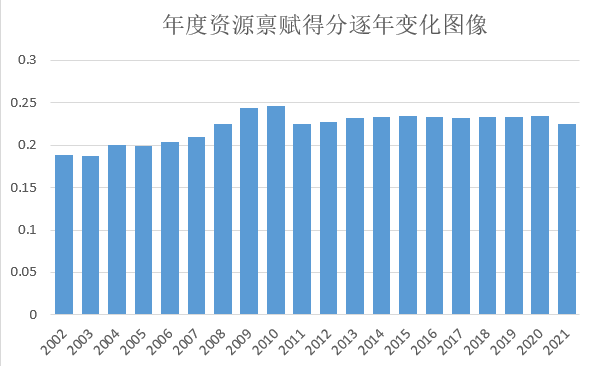
\includegraphics[width=6cm]{pictures/zybfdf.png}
		\caption{资源禀赋得分}
		\label{zybfdf}
	\end{figure}
	\newpage
	\leftline{教育水平得分}
~\\0.068248304
\quad 0.078376808
\quad 0.088792191
\quad 0.098471039
\quad 0.109189945
\quad 0.121752831
\quad 0.134848033
\quad 0.148004027
\quad 0.158609029
\quad 0.176466134
\quad 0.199462104
\quad 0.207611471
\quad 0.221510795
\quad 0.254308978
\quad 0.271458086
\quad 0.285425559
\quad 0.298060768
\quad 0.314331933
\quad 0.342770703
\quad 0.38112215
	\begin{figure}[htb]
	\centering
	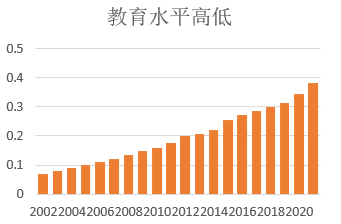
\includegraphics[width=6cm]{pictures/jyspdf.png}
	\caption{教育水平得分}
	\label{jyspdf}
	\end{figure}
	\\\leftline{人口规模得分}
~\\	0.211906864
\quad	0.212906214
\quad	0.21515997
\quad	0.219274112
\quad	0.220776243
\quad	0.222037004
\quad	0.223490431
\quad	0.224859723
\quad	0.230028793
\quad	0.230413202
\quad	0.230435218
\quad	0.230574176
\quad	0.229875682
\quad	0.229257781
\quad	0.228526494
\quad	0.227035536
\quad	0.225619917
\quad	0.224141214
\quad	0.217968714
\quad	0.215675706
	
	\begin{figure}[htb]
	\centering
	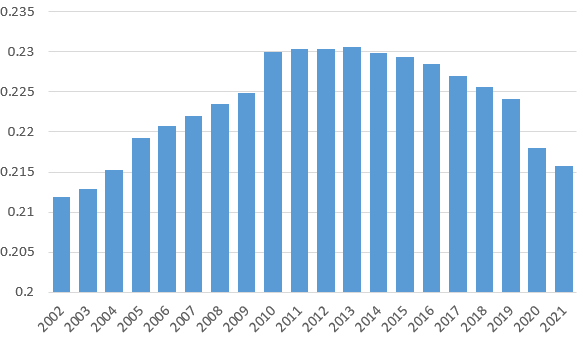
\includegraphics[width=6cm]{pictures/rkgmdf.png}
	\caption{人口规模得分}
	\label{zybfdf}
	\end{figure}
	\leftline{外商投资得分}
~\\0.1079
\quad 0.1094
\quad 0.1240
\quad 0.1234
\quad 0.1289
\quad 0.1529
\quad 0.1890
\quad 0.1841
\quad 0.2163
\quad 0.2373
\quad 0.2285
\quad 0.2405
\quad 0.2445
\quad 0.2583
\quad 0.2577
\quad 0.2680
\quad 0.2760
\quad 0.2825
\quad 0.2953
\quad 0.3393

	\begin{figure}[htb]
	\centering
	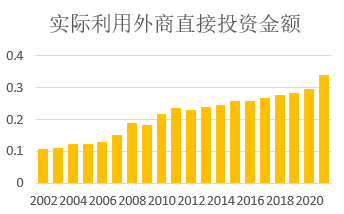
\includegraphics[width=6cm]{pictures/wstzdf.png}
	\caption{外商投资得分}
	\label{wstzdf}
	\end{figure}
	\subsection*{II 支撑材料文件列表}
	\begin{itemize}
		\item 分类原始数据.rar
		\item 原始数据汇总.xls
		\item 建模求解分析过程草稿.docx
		\item 数据处理过程,结果及代码.docx
	\end{itemize}
\end{document}